{\Huge{}{ \textbf{\exc \  }}}

{\Huge{}{ \textbf{Fusion Modelling System Science Plan} }}

\section*{Purpose}

This document outlines the Science Plan for research to be commissioned 
by the Met Office for the ``Fusion Modelling System'' use case of the SPF ``\textbf{Ex}ascale 
\textbf{C}omputing \textbf{Al}gorithms 
and \textbf{I}nfrastructures \textbf{B}enefiting 
\textbf{U}K \textbf{R} esearch'' 
programme (\exc \  ). It complements \exc \   Met Office Science Plan and Activities 
document [1], setting out a vision for the project's contribution to the overarching 
\exc \   plan. This document is aimed at stakeholders including the SPF \exc \   
Programme Board and Steering Committee, has been informed by consultation with 
the Met Office, with domain experts from across the UKRI community and from within 
UKAEA. This Science Plan is intended to complement other \exc \   work funded 
through the UKRI Research Councils and the Met Office ``Weather \& Climate Prediction'' 
use case.

\textit{The \exc \   programmatic aims described in [1] are common 
with those of the Fusion Modelling System use case and so are not repeated here.}

\section*{Fusion Modelling Use Case activities}

The aim of the ``Fusion Modelling'' use case of \exc \   
is, via the exploitation of the \exc \   principles outlined in [1], to develop 
new algorithms, software and related e-Infrastructure that will result in the efficient 
use of current Petascale and future Exascale supercomputing hardware in order to
\begin{enumerate}
\item draw insights from ITER [2] ``Big Data'' 
\item to guide and optimise the design of the UK demonstration nuclear fusion
power plant STEP [3] and related fusion technology
\end{enumerate}
as we approach the Exascale. The aims of the work are to deliver expertise 
in, and tools for, ``in-silico'' reactor interpretation and design, initially with 
a focus upon the ``edge'' region of the tokamak [4] plasma where hot plasma comes 
into contact with the material walls of the machine (see project \nep \   below). 
This challenging, multi-physics, multi-scale intersection between plasma physics 
and engineering has long been heralded as an ``exascale'' modelling and simulation 
problem and its solution is well established as critical to the success of commercial 
fusion energy. Existing legacy (and often ``black box'') codes do not scale and 
do not contain all the latest physics that is believed to be important in the ``burning 
plasma regime'' (notably kinetic effects); without a significant investment in 
this area, it will not be possible to design the ``divertor'' region of future 
fusion power plants (the region of the machine where hot plasma comes into contact 
with the surrounding first wall - see Figure 1 below).

\begin{figure}[htbp]
\centerline{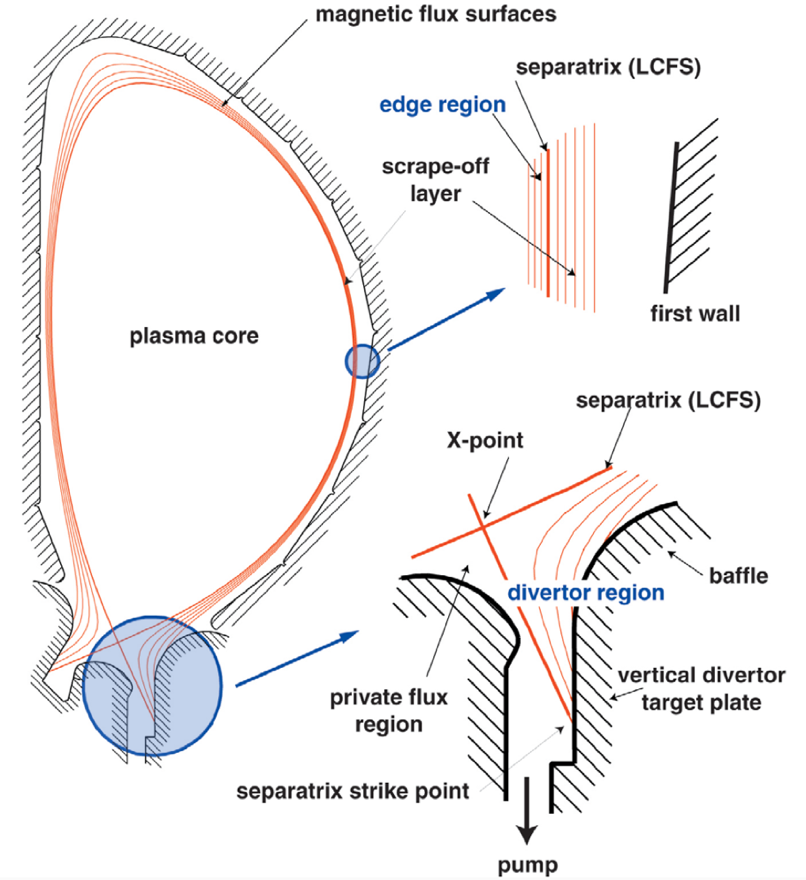
\includegraphics[width=261pt, height=285pt, keepaspectratio=true]{../corpics/edge_geometry.png}}
\caption{Schematic diagram of a generic tokamak ``poloidal 
cross section'' showing the areas of plasma and first wall that will be targeted 
by project \nep \   (shaded circles). Attribution: G. Federici et al. [CC BY 3.0 
( \url{https://creativecommons.org/licenses/by/3.0}),
minor modifications to figure]. }
\end{figure}

This is an activity that must be performed ``in-silico'' 
using ``actionable'' modelling and simulation as the highly coupled physics in 
the divertor cannot be created in the laboratory with conditions approaching the 
reactor regime. It is also well established that there is a need for further development 
of the science (which will take place in close cooperation with \exc \   numericists) 
- the codes of the ITER and Exascale era must therefore be easy to adapt as new 
knowledge becomes established (eg.\ through ITER operations). The programme itself 
is designed to exploit commonality of solutions across the disciplines and domains 
represented by \exc \   and to foster the development of a UK interdisciplinary 
community (within our National laboratories and institutes across UKRI and throughout 
Academia).

Activities will initially be around an ambitious programme to develop a computational 
model that includes plasma kinetic effects believed to be essential for a first-principles 
description of the complex dynamics of high temperature fusion plasma in the divertor 
region.  Codenamed \nep \   ( \textbf{NE}utrals \&  \textbf{P}lasma  \textbf{TU}rbulence 
\textbf{N}umerics for the  \textbf{E}xascale), 
work will initially focus upon coupling the turbulent plasma periphery to the surrounding 
neutral gas and partially ionized impurities that exist between the plasma and 
plasma facing components, in the presence of an arbitrary tokamak magnetic field 
and full 3-D first wall geometry. Figure 1 shows a schematic of a generic tokamak 
``poloidal cross section'', highlighting the targeted regions of plasma and machine, 
namely the main chamber between
core plasma scrape off layer and wall (upper shaded circle) and the so called ``plasma
exhaust" or ``divertor" region (lower shaded circle) where heat and particles come into direct
contact with material surfaces. Infrastructure and workflows will be developed so that the
resulting close coupled
models can be constructed routinely based around a high-fidelity representation 
of the geometry described by Computer Aided Design (CAD) systems (this likely requiring 
the development of high order meshing technology, eg.\ using Nektar++).

Quality control, verification, validation and uncertainty quantification 
(VVUQ, eg.\ via intrusive or ensemble-based methods) will be embedded across all 
areas of the project to ensure numerical predictions are ``actionable''. The initial 
aim is to develop knowledge and UK capability around how to design world leading 
Exascale targeted software for the benefit of the UK academic community, UKRI and 
the UK nuclear supply chain. Emphasis will be placed upon building a connected 
community, delivering training and skills development activities as necessary, 
aligned with Pillar 4 of the \exc \   aims (Investing in People).

Together, the UK plasma and HPC communities have the required expertise to deliver 
this project. UKAEA will bring together world-class experts in tokamak edge physics, 
gyroaveraged kinetic theory, and highly scalable algorithms, to address arguably one of 
the most important unsolved challenges of fusion research - how to design a plasma 
``exhaust system'' that can reliably restrict power flux reaching the material 
surfaces to tolerable levels, ie.\ no more than \textasciitilde{}10MW/m\textsuperscript{2} 
in the steady-state. Later in the project, further packages of work will be designed 
to address other aspects around the ``in-silico'' design of fusion technology. 
It is recognised that the project poses a significant human resource and project 
management challenge, notably to develop and manage a team across many different 
sites and from many different backgrounds in order to build state-of-the-art software 
that can reliably and accurately account for a plethora of different complex physical 
phenomena. Further, the project must maintain an international context and connect 
to the European EUROfusion programme (in which the UK is a key player) and the 
US Exascale programme (ECP). Crucially, the emerging software environment must 
be trusted and ``actionable'' to guide procurements potentially involving hundreds 
of millions of pounds (eg.\ in the case of the  DEMO [5] first 
wall), and ultimately to ensure the safe operation of a multi-billion pound nuclear 
plant.

The UK is world-leading in the study of the edge region of tokamak plasmas. The 
flagship EPSRC/EUROfusion MAST-Upgrade experiment [6] recently 
commissioned by UKAEA at Culham has been built with the primary goal of testing 
a novel ``Super-X divertor'' design for handling the plasma exhaust. Combined with 
software developed under \exc \  , the result will be a significant step forward 
in our understanding of how heat and particle flows can be controlled and kept 
to within material limits inside a reactor.

\section*{{\huge{}{ \textbf{Project \nep \  }}}}

\textbf{(}{\textbf{NE}}\textbf{utrals \& }{\textbf{P}}\textbf{lasma 
}{\textbf{TU}}\textbf{rbulence }{\textbf{N}}\textbf{umerics 
for the }{\textbf{E}}\textbf{xascale) - background}

The UK plasma community - in UKAEA and several universities - currently makes extensive 
use of ``fluid'' codes in its research into the edge-plasma region of fusion devices. 
``Fluid'' implies that the plasma can be treated in one sense like ``the atmosphere'' 
in the Met Office's Dynamical Core, but with the added complication of significant 
effects due to the electrically charged nature of the plasma. For example, plasma 
electrons and ions can to an extent be treated as separate fluids with different 
temperatures, interacting via the electromagnetic field. Plasma fluid codes (such 
as  BOUT++ [7]) are relatively efficient up to only \textasciitilde{}1000 
cores, but there are a large range of effects in the tokamak plasma edge that prevent 
the plasma from isotropising to a Maxwellian distribution with same temperature 
ion and electron populations (which would correspond most closely to the atmospheric 
fluid concept). Firstly, the strong imposed and directed magnetic field leads to 
anisotropy since charged particles move rapidly in tight, spiral orbits (gyro-orbits) 
along the closed field lines and only slowly normal to the field. Secondly there 
may be an inadequate number of collisions (especially in the burning plasma or 
``reactor'' regime) for the species to equilibrate, leaving significant tails in 
the particle velocity distributions. Such tails may be driven by external heating 
and/or by collisions with relatively rarefied neutral particle species that are 
themselves non-Maxwellian. Inclusion of these effects in the fluid models introduces 
significant modelling uncertainty (which would have to be quantified if the models 
are to be ``actionable'' - this would require a significant investment). Moreover, 
existing simulations show that attempting to include the required extra physics 
can significantly add to execution cost overhead or a breakdown of scaling, eg.\ 
when stability/accuracy issues are addressed, a large reduction in allowable timestep 
can ensue. Unfortunately, there are significant challenges with moving to a straightforward 
particle-based  model (eg.\ PIC [8], which could in principle 
address these problems) - the strength of the electric field in the plasma edge 
exaggerates the effects of noise when sampling charged particles. Together, all 
these issues conspire to make it impossible to achieve converged solutions using 
existing codes within an acceptable timeframe.

The next most widely studied level of treatment of velocity space,  namely 
``gyrokinetics'' [9], averages over gyro-orbits so that velocity space is treated 
as a 2-D problem (perpendicular and parallel to the local magnetic field). This 
leads to 5-D gyroaveraged models, which in principle are detailed enough and accurate 
enough to model reality. Ideas around the discretisation of the velocity (phase) 
space dependence include techniques suitable for dealing with infinite coordinates, 
such as moment-based methods using truncated series and/or mapped finite elements 
perhaps combined with spherical harmonics. The alternative, particle-based simulations 
that run on existing petascale hardware such as SUMMIT, eg.\ using the XGC PIC 
code, can take many weeks for just a single simulation. Unfortunately, the competing 
and potentially more attractive 5-D gyroaveraged models are currently at or beyond 
the limit of current HPC capability in terms of scalabiliy, requiring further work 
around both the models themselves and the algorithms used to instantiate them on 
modern HPC systems.

Kinetic levels of complexity are nonetheless going to be necessary (at least locally) 
for modelling the burning plasma regime, due to the inherent uncertainty in the 
fluid codes. The plasma in a fusion reactor may well behave significantly differently 
to plasma in existing devices because it will in general contain two main ionic 
species (Deuterium and Tritium), neutral fuel particles and ionised Helium ash 
(or alpha particles), as well as impurity ions originating from the wall. Further, 
the plasma will be hotter, reducing collisions so that yet more complicated terms 
need to be added to the fluid approximations. These additional contributions to 
the fluid models will require tuning in much the same way as meteorological micro-physical 
effects, but in advance preferably of suitable experimental data from ITER or other 
reactors. Kinetic code results will inevitably be needed for this ``tuning'' exercise 
(ie.\ providing kinetic closures to the fluid codes). Each plasma species will 
contribute different levels of uncertainty, and a different scaling and performance 
overhead to the workflow made up of close coupled codes that will be developed 
under FM-WP2 and FM-WP3 (see below and Table 1). Identifying, quantifying and mitigating 
uncertainty and the computational overhead of adequately modelling each will be 
a core theme within the project.

Evidently the interpretation of data from ITER and consequently the design of a 
DEMO fusion power plant will require a hierarchy of models, from those that can 
be deployed upon Exascale hardware down to the surrogate models that will be deployed 
at scale upon the high throughput computing platforms of the ITER era (eg.\ for 
uncertainty quantification and parametric optimisation). High fidelity, exascale 
``hero run'' codes capable of modelling all the required physics to accurately 
describe the edge region of the tokamak plasma will be used to develop order reduced 
``surrogate'' models that can be scaled out for testing against large volumes of 
experimental data and for routine uncertainty quantification as part of the process 
shown in Figure 2 (left hand branch). Currently, this iterative ``discovery loop'' 
is not possible for the edge plasma problem due to the unacceptable run-time overhead 
of existing codes and lack of flexibility for introducing new physics. Similarly, 
the high fidelity and surrogate models of the future will be crucial for designing 
future fusion plant ``in-silico'' (this is shown as the right-hand branch of Figure 
2 - an iterative ``optimization'' loop). 

\begin{center}
\begin{figure}[htbp]
\centerline{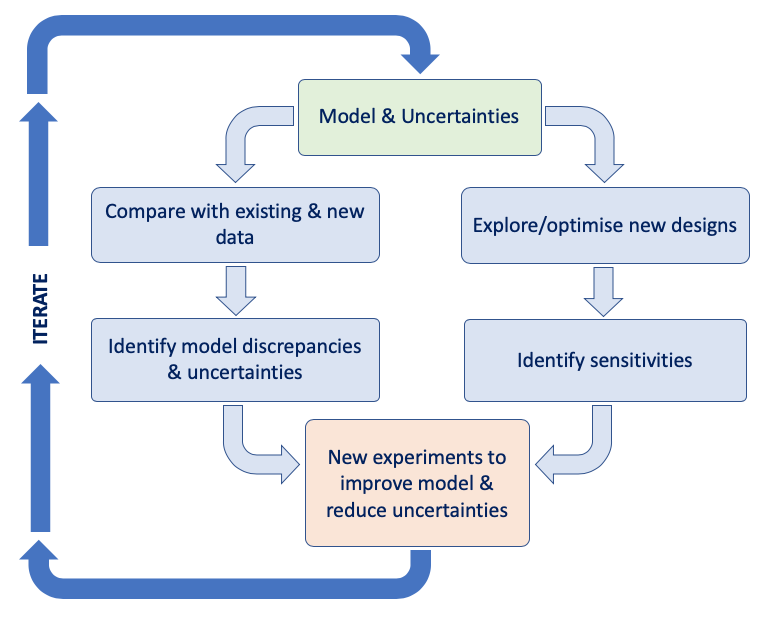
\includegraphics[width=332pt, height=265pt, keepaspectratio=true]{../corpics/UQflow.png}}
\caption{Typical ``Modelling \& Simulation'' workflow for fusion applications. 
The left-hand iterative loop is largely around model validation against experimental 
data whereas the right-hand loop focuses upon ``engineering design''.}
\end{figure}
\end{center}

The existing code base is currently limited in its ability (for the same reasons 
as the left-hand branch) to make accurate predictions that will lead to robust 
engineering solutions (leading to the introduction of unnecessary and expensive 
engineering overhead). The current paradigm is to make predictions, then build 
expensive prototypes at scale to confirm that the code predictions are valid - 
this will be impossible for STEP and DEMO for cost reasons and due to the fact 
that we simply cannot recreate the operating conditions under which components 
will have to survive - instead, quantified uncertainty and ``trust'' must be associated 
with modelling and simulation through rigorous, modern VVUQ - ie.\ our codes must 
be ``actionable''. Lastly, there are also likely to be additional demands upon 
code execution speed from DEMO operation, for example there will inevitably be 
a safety-related need for surrogate models that can be deployed as part of future 
real-time systems to help control the temperature of the first wall. These future 
needs will all be embedded within the heart of the project requirements throughout 
the development lifecycle of the \nep \   software stack. 

The project itself has been designed in stages, so that early work will make significant 
contributions to existing software capability and to the development of standalone 
\papp s  [10] that capture the scaling characteristics of the 
full models being targeted in the long term. The overall aim, which will guide 
the direction of the project and choice of Activites and sub-tasks (most of which 
will be defrayed across UKRI and the Universities), is to build a hierarchy of 
models that are capable of representing edge plasma behaviour to within a specific 
level of uncertainty, with the option of at least partial incorporation into the 
development of software across the EUROfusion work programme, notably the TSVV 
(Theory, Simulation, Verification and Validation) activities. There will be no 
attempt to refactor or improve the performance of existing legacy codes (unless 
the overhead of doing so is low). Instead, emphasis will be upon building new insight/knowledge 
and new software and infrastructure from the ground up using modern software engineering 
design principles and futureproofing those tools to create an agile platform that 
can respond to the rapidly changing vision of what the exascale will look like, 
and to the emergence of new physics understanding. All codes that are capable of 
making predictions will have embedded within them the concepts of VVUQ, to ensure 
that they are ``actionable'' to within specified levels of uncertainty (eg.\ using 
``intrusive'' UQ methods). Existing legacy codes will of course be an invaluable 
resource for guiding development towards the flexible, scalable and performant 
codes of the future.

High level aims of the \exc \   Fusion use case, aligned with the Met Office Weather 
\& Climate prediction system use case include:

\begin{itemize}
\item[$\bullet$] To apply the principles of \exc \   to deliver the benefits outlined above.

\item[$\bullet$] To develop and deliver cross-cutting research that aligns with the UKRI Research 
Council contribution (ie.\ to help deliver a UK interdisciplinary team that can 
address aspects of Exascale software design that lie in common across the represented 
use cases).

\item[$\bullet$] To help train the software engineers, architecture specialists, computer scientists/algorithms 
specialists and data scientists of the ITER and Exascale era.
\end{itemize}

UKAEA will work with the SPF \exc \   Programme Board and Steering Committee to 
ensure alignment and a close working relationship with the UKRI funded research 
activities, which for example could include participation in workshops and knowledge 
exchange activities, participation in stakeholder engagement exercises etc.

As part of this Science Plan, four work packages will initially be commissioned 
by the Met Office, ie.\ FM-WP1/2/3/4. As outlined in the Met Office Science Plan 
[1], the Met Office will manage the cross-cutting theme work packages XC-WP1/2 
(see below). The four initial Fusion Modelling System work packages are:

\begin{enumerate}
\item Numerical representation;

\item Plasma multiphysics model;

\item Neutral gas \& impurity model;

\item Code structure and coordination,
\end{enumerate}

as shown in Table 1 (and in [1]). Code Coupling R\&D activity will thread FM-WP1 
(performance) and FM-WP4 (flexibility) as well as through the two referent model 
work packages FM-WP2 and FM-WP3. All work packages will be built around modern 
best practice in co-design and there will be significant interaction between the 
work packages. Each work package will be supported by Research Software Engineers (RSEs) (including
engagement with the Society of RSE [11] where necessary).

\begin{center}
\begin{table}[h]
\footnotesize
\begin{tabular}{|>{\raggedright}p{76pt}|>{\raggedright}p{63pt}|>{\raggedright}p{79pt}|>{\raggedright}p{69pt}|>{\raggedright}p{66pt}|}
\hline
\multicolumn{5}{|p{353pt}|}{\textbf{PSRE Use Cases}}\tabularnewline
\hline
Weather \& Climate prediction system: & \multicolumn{2}{p{142pt}|}{\textbf{WC-WP1:}\linebreak{}
Component model co-design} & \textbf{WC-WP2:}\linebreak{}
System co-design & \textbf{WC-WP3:}\linebreak{}
System integration\tabularnewline
\hline
Fusion Modelling system: & \textbf{FM-WP1:}\linebreak{}
Numerical representation & \textbf{FM-WP2:}\linebreak{}
Plasma multiphysics model & \textbf{FM-WP3:}\linebreak{}
Neutral gas \& Impurity model & \textbf{FM-WP4:}\linebreak{}
Code structure \& coordination\tabularnewline
\hline
\multicolumn{5}{|p{353pt}|}{\textbf{Cross-Cutting Themes}}\tabularnewline
\hline
\multicolumn{2}{|p{142pt}|}{\textbf{XC-WP1:}\linebreak{}
Common approaches \& solutions} & \multicolumn{3}{p{217pt}|}{\textbf{XC-WP2:}\linebreak{}
Emerging technologies}\tabularnewline
\hline
\end{tabular}
\normalsize
\title{Table 1: SPF \exc \   Met Office commissioned Work Packages.}
\end{table}
\end{center}

\baselineskip=12pt
\textbf{FM-WP1} will focus upon the suitability of available numerical algorithms 
(or the development of new algorithms) for Exascale targeted plasma modelling. 
As stated above, elements of this work package together with FM-WP4 will also surround 
the ``coupling technology'' that will be required to connect the edge/pedestal 
region of the plasma (addressed by FM-WP2) and the neutral gas/impurity model (FM-WP3). 
An agile approach will be adopted around the legacy codes that might be necessary 
for helping to develop a roadmap for the FM-WP1 referent models, eg.\ through community 
workshops (the first being in Feb 2020).

\textbf{FM-WP2} and \textbf{FM-WP3} will concentrate upon development of the two 
close coupled models of the \nep \   programme, specifically FM-WP2 around the inclusion 
of kinetic effects into existing and new edge plasma models, and FM-WP3 of particle 
based models for describing the region outside and just inside the plasma (neutral 
atoms/molecules and partially ionized impurities). Initial exploratory work will 
be carried out using existing codes (as per above) and via the development of \papp s, 
for example to expose options for exascale targeted hardware (GPUs, ARM technology 
etc.).

\textbf{FM-WP4} will focus upon the design of data structures to interface between 
the different models and generally ensure best practice in scientific software 
engineering (being responsible for Quality Assurance, co-design, integration etc.). 
Aligned with Met Office work package WC-WP1, this programme of 
work will also explore the use of a ``separation of concerns'' methodology for 
the Fusion use case critical components (eg.\ by exploring the use of Kokkos [12] 
and Domain Specific Language (DSL) [13] technologies).

Scoping work for the Met Office led cross-cutting themes (XC-WP1 and 2) will be 
defined in collaboration with the other \exc \   partners early in year 2 with 
a view towards starting work later that year. The specifics of the cross-cutting 
themes are here assumed to be covered by the two overarching themes of ``Common 
Approaches and Solutions'' and ``Emerging Technologies'' (discussed further below).

Note, many of the Activities and sub-tasks that will be defrayed to UKAEA, the 
Universities and UKRI (STFC) will inevitably contribute to more than one of the 
overarching Work Packages due to the highly coupled nature of the target infrastructure.

\section*{{\huge{}{\textbf{UKAEA Research Plans}}}}

\subsection*{\textbf{Numerical representation (} Fusion modelling, work package  \textbf{FM-WP1})}

The ideal numerical algorithms for forming the Exascale edge plasma codes of the 
future will have (but will not be restricted to) the following properties:

\begin{itemize}
\item[P1.] Accurate solution of hyperbolic problems.

\item[P2.] Ability to deliver efficient and accurate solutions of corresponding elliptic 
problems.

\item[P3.] Accurate modelling of highly anisotropic dynamics. 

\item[P4.] Accurate representation of first wall geometry (face normals to within 0.1°), 
and correspondingly of complex magnetic field geometries.

\item[P5.] Accurate representation of velocity (phase) space.

\item[P6.] Preservation of conservation properties of the underlying equations.

\item[P7.] Scalability to likely Exascale architectures:

\begin{enumerate}
\item interaction between models of different dimensionality,

\item interaction between particle and fluid models,

\item dynamic construction of surrogates.
\end{enumerate}

\item[P8.] Performance portability to allow rapid deployment upon emerging hardware.
\end{itemize}

It is difficult at this point in time to rank the importance of these properties, 
or to identify the cost associated with achieving each in a timely fashion - a 
clearer understanding of immediate needs and achievable SMART deliverables will 
emerge as the project matures via extensive community engagement and team building 
across the UK partners - this exercise will start in Feb 2020 via an open workshop. 

It is clear however that the choice of geometrical representation and numerical 
scheme will have a profound impact upon almost all areas of the project. Options 
will be identified by means of literature and code surveys and via consultation 
with UKRI and industry experts. Research will be commissioned where necessary to 
eliminate unsuitable choices as early as possible. Relatively small development 
tasks will initially be undertaken to test remaining candidate methods for accuracy, 
stability and HPC scalability potential.  This task, along with FM-WP4 will have 
a prioritised start to provide initial inputs into FM-WP2 and FM-WP3 developments 
and work to be defrayed in year 2. Tasks FM-WP1-3 will incorporate numerical, finite 
element and other plasma physics libraries of suitable quality and exascale applicability.

Options, which do not preclude consideration of others, have 
been tentatively identified for initial investigation as follows:

\begin{enumerate}
\item Spectral/hp element [14], combined with Discontinuous  Galerkin 
[15], to meet P1,P3 and possibly P5 above.

\item Multigrid methods for P2.

\item Nekmesh for P4.

\item For the Exascale (P7):

\begin{enumerate}
\item matrix-based approaches, hierarchical geometric structures,

\item kinetic enslavement, multi-index Monte-Carlo methods,

\item physics based Neural Network approaches.
\end{enumerate}

\item MUSCLE 2 etc. as referenced in [16], MUI [17], ADIOS [18] etc. 
for code coupling P6, P7.
\end{enumerate}

As per the algorithm requirements, these will be ranked via the community workshop 
planned for Feb 2020. Activities for defrayment will then be defined around SMART 
deliverables together with an integrated delivery plan for the entire project.

\subsection*{\textbf{Plasma multiphysics model} (Fusion modelling, work package \textbf{FM-WP2})}

This work package will begin by identifying a referent in conjunction with potential 
users, whereby ``referent'' is meant a model that establishes the maximum detail 
and complexity of plasma that the software could ever be reasonably expected to 
model (beyond exascale).  Critical features of the referent will be identified 
and prioritised for implementation as part of the project. This may involve replacing 
a kinetic model by moment-based or fluid models. Input from the European Boundary 
Code (EBC) development (funded by EUROfusion wherein UKAEA is a core partner) will 
be important to this process. In addition, the speed of model execution will be 
a consideration as indicated earlier. A provisional sequence of developments is 
as follows (and will be tuned as part of the initial \nep \   requirements capture 
exercise funded in year 1):

\begin{enumerate}
\item 2-D model of anisotropic heat transport.

\item 2-D elliptic solver in complex geometry.

\item 1-D fluid solver with simplified physics but with UQ and realistic boundary conditions.

\item Spatially 1-D plasma model incorporating velocity space effects.

\item Spatially 1-D multispecies plasma model.

\item Spatially 2-D plasma model incorporating velocity space effects.

\item Interaction between models of different dimensionality.

\item Spatially 3-D plasma kinetic models.
\end{enumerate}

Users from the wider fusion community will be engaged via a workshop in Feb 2020 
to firm up on the plan, to help define work for defrayment that they themselves 
can carry out and will be engaged throughout the project to help define and add 
new surrogate models through a wide engagement programme and co-design (eg.\ to 
treat boundary sheaths) and/or other important physical effects (eg.\ radiation, 
charge exchange recombination, etc.) and compare with existing codes and experiments. 


\subsection*{\textbf{Neutral gas \& Impurity model}  (Fusion modelling, work package  \textbf{FM-WP3})}

This work package will begin by identifying a referent (as above) in conjunction 
with potential users and experts in atomic physics. Critical features of the referent 
will be identified and prioritised for implementation as part of the project. This 
may involve deploying a particle-based method, a moment-based model or a fluid 
model (or even a combination thereof). Input from the European EBC programme will 
be important to this process, as will the speed of model execution as indicated 
earlier. A careful assessment of existing codes currently in use will 
be necessary, as will cross validation with the established models (notably B2-EIRENE 
[19]). A provisional sequence of developments is as follows:

\begin{enumerate}
\item 2-D particle-based model of neutral gas \& impurities with critical physics.

\item 2-D moment-based model of neutral gas \& impurities.

\item Interaction with 2-D plasma model when available.

\item 3-D model of neutral gas \& impurities.

\item Interaction with 3-D plasma model.

\item Staged introduction of additional neutral gas/impurity physics.
\end{enumerate}

As per FM-WP2, users from the wider fusion modelling community will first be engaged 
through a workshop in Feb 2020, and will help build a UK team that will add new 
physics and compare with existing codes and experiments, providing detailed and 
rigorous verification and validation (V\&V). This is likely to require the provision 
of databases for different ionisation and excitation reactions, both in the plasma 
volume and at surfaces.

\subsection*{\textbf{Code structure and coordination} (Fusion modelling, work package \textbf{FM-WP4})}

The most important aim of this work package will be to drive user engagement and 
ensure that the software is fit for its defined purpose, first by requirements 
capture, then by defining suitably flexible code structures and related e-Infrastructure 
for users, ultimately supporting uptake of the new code(s). In order to achieve 
this aim, this work package will coordinate across the other tasks FM-WP1-3, to 
ensure that outcomes are compatible and of sufficiently high quality. There will 
be management and coordination tasks that will grow as the project matures, connecting 
with the EUROfusion E-TASC (TSVV) programme, the EPSRC T.P. Turbulence Programme 
[20] and the US ECP programme etc.

Coordination tasks will include (but are not restricted to):

\begin{enumerate}
\item Allocation of resource between tasks and setting project priorities.

\item Ensuring a consistent choice of definitions (ontology) of objects or equivalently 
classes.

\item Definition of common interfaces to components for data input and output. 

\item Design of suitably flexible data structures for common use by all developers.

\item Establishment, promotion and support of good scientific software engineering 
practice.

\item Evaluation and deployment of performance portability tools and DSLs targeting 
Exascale-relevant architectures.

\item Integration of the developed software into a VVUQ framework (exploiting common 
approaches developed under XC-WP1 and XC-WP2).

\item Coordination of a benchmarking framework for correctness testing and performance 
evaluation of the developed software stack.
\end{enumerate}

Along with FM-WP1, this work package will be prioritised for an early start, as 
good scientific software engineering practice needs to be agreed quickly, and well 
documented interfaces to components need to be available early to ensure that best 
practice design is embedded from the start.


\subsection*{\textbf{Common approaches and solutions} (Cross-cutting themes,  \textbf{XC-WP1})}

The examples listed in [1] are very well aligned with the needs 
of the Fusion use case comprising initially \nep \  , especially the methodologies 
surrounding a ``separation of concerns'', coupling technologies, the use of mixed 
precision arithmetic and fault tolerance. In addition, project \nep \   will benefit 
from an exploration of the convergence of HPC and AI (eg.\ the use of Neural Network 
PDE solvers [21] or for advanced preconditioners) and parallel in time methods 
[22]. These areas of common ground and opportunities for interdisciplinary working 
therein shall be explored and agreed by partners as outlined in the Met Office 
Science Case.

\subsection*{\textbf{Emerging Technologies}  (Cross-cutting themes, \textbf{XC-WP2})}

The examples listed for XC-WP2 in the Met Office Science Case 
[1] are again highly aligned with the Fusion use case. Other technologies that 
are deserving of consideration include High Bandwidth Memory (HBM [23]), novel 
exascale targeted IO/storage technology (eg.\ H2020 project SAGE II [24] led by 
Seagate wherein UKAEA is a partner), next generation accelerator technology (Nvidia 
Volta Next, A64fx) and ARM systems for efficient scaling of Flops/Watt. It is not 
clear at this stage which technologies offer the best route forward for the FM-WP2 
and FM-WP3 close coupled system but it is clear that the UK is well placed to explore 
all of them (eg.\ through Isambard II). As stated earlier, a core theme within 
the project is to build solutions around a ``separation of concerns'' philosophy 
(using tools such as Kokkos and One-API) in order to develop an agile environment 
that can adapt rapidly to disruptive emergent HPC technology.
